
\section{Resolución}
\subsection{Organización}
Organización temporal y de trabajo

\subsection{Desarrollo}
Desarrollo y resolucion completa

\subsubsection{Entrenamiento}
En esta fase del KDD, se eligieron y entrenaron diferentes modelos matemáticos para el análisis del set de datos. El objetivo del proyecto es conseguir predecir las etiquetas de las señales de sonidos no verbales, para ello se entrenaron los siguientes modelos:
\begin{itemize}
    \item K-vecinos más cercanos (KNN)
    \item Redes de neuronas artificiales secuenciales (SNN)
\end{itemize}
Ambos algoritmos son supervisados, para la clasificación de datos nuevos se entrena al modelo con datos etiquetados y el modelo aprende en función de si ha clasificado bien o mal datos etiquetados.

La idea básica detrás de KNN es que los puntos de datos similares tienden a agruparse en el espacio de características. Cuando se clasifica un nuevo punto de datos (en este caso, un nuevo audio), el algoritmo busca los "K" puntos de datos más cercanos (vecinos) en el espacio de características. Luego, asigna la clase más común entre esos vecinos al punto de datos de prueba. Para KNN se obtuvieron resultados poco satisfactorios con precisiones inferiores al 50\%. Aunque es posible que se pudieran obtener mejores resultados, utilizando representaciones de los datos como espectrogramas basados en los coeficientes cepstrales de Mel, se tomó la decisión de abordar el problema de clasificación principalmente con redes neuronales artificiales.

Las redes neuronales en el contexto del aprendizaje automático (machine learning) son un tipo de modelo computacional inspirado en la estructura y el funcionamiento del cerebro humano. Están compuestas por unidades de procesamiento llamadas neuronas artificiales que están organizadas en capas y conectadas mediante conexiones ponderadas. Las redes neuronales articificiales o redes neuronales secuenciales (en adelante RNA), son excelentes en la clasificación de sonidos por ser capaces de aprender características complejas de los datos, su flexibilidad en la representación de datos y adaptabilidad, esto las convierte en clasificadores consistentes aprueba de fallos como pueden ser incompletitudes en los datos.

Se comenzó realizando arquitecturas secuenciales con capas densas. Las capas densas son un tipo de conexiones entre neuronas que conectan todas las neuronas de entrada con todas las de salida, y de manera automática utilizando regresores lineales ajustan mediante pesos como de importante es cada conexión. Este tipo de capas tienen la desventaja de que estudian de manera parcial el orden en el que aparecen los datos, y los sonidos que se pretenden estudiar tienen carácteristicas que son temporalmente dependientes, como puede ser tras una tos un sonido de inspiración o la variación en amplitud al final de la misma. Se probaron modelos más simples con pocas capas y más complejos con muchas capas. Los resultados fueron peores que los obtenidos con KNN y además el modelo se encontraba limitado por su arquitectura, no superando el umbral de 25\% a pesar de aumentar el número de capas.

Viendo los resultados anteriores, se probó con modelos basados en capas convolucionales unidimensionales, esta arquitectura permite a la red extraer información posicional de los eventos que ocurren en los audios, este tipo de capas utilizan múltiples filtros sobre ventanas de los vectores de amplitudes, obteniendo diferentes mapas de características. La finalidad de estas capas es reducir la dimensionalidad de los audios, llevando el espacio de dimensiones a otras más facilmente interpretables por regresores lineales.
La mejora al usar este tipo de modelos fue notable, tanto modelos sencillos como más complejos, el mejor modelo alcanzado en mayo de 2024 tuvo un precisión del 85\%, a continuación se muestra la tabla parámetros entrenables de la mejor arquitectura:
\begin{center}
    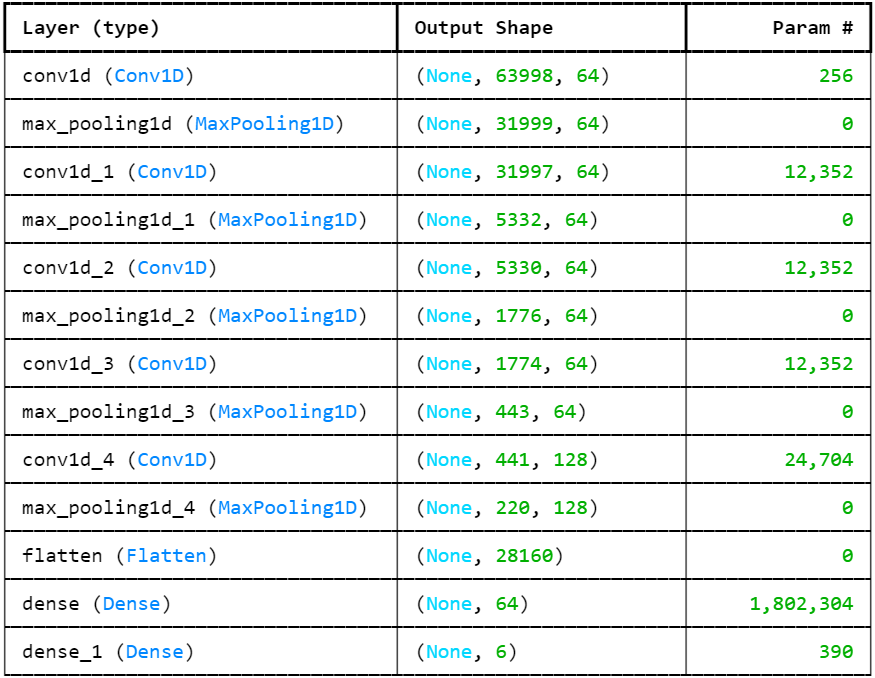
\includegraphics[width=0.8\textwidth]{ImagenesLatex/Conv1D_capas.PNG}
\end{center}
Los hiperparámetros principales para este modelo:

Una vez se definió la arquitectura se estimaron los hiperparámetros para cada modelo, se utilizaron para todos los modelos de RNA los siguientes:
\begin{itemize}
    \item Train(\%), Test(\%): 80\%, 20\%
    \item Batch size: 128 (máximo permitido por colab)
    \item Learning rate: Variable entre 0.01 y 0.001
    \item Epochs: dependiente del modelo
\end{itemize}
Para el mejor modelo el número de épocas fue 12.
\subsubsection{Comparativa de modelos}
Por simplicidad para la comparativa de modelos se tuvo en cuenta principalmente su precisión para resolver el problema en cuestión, se deja como trabajo a futuro el estudio en escalabilidad y ocupación en memoria de los parámetros entrenados.

Para la elección del modelo que se usará para la implementación real, se compararon los siguientes resultados:
\begin{center}
    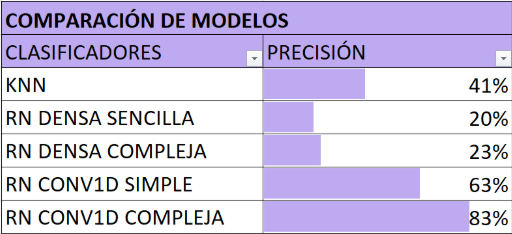
\includegraphics[width=0.8\textwidth]{ImagenesLatex/ComparacionModelos.PNG}
\end{center}

El mejor modelo obtenido en abril de 2024 fue el realizado con capas convolucionales 1D, que por tener más de 2 capas entra en la categoría de deep learning.
